\begin{figure}[htbp]
  \centering
  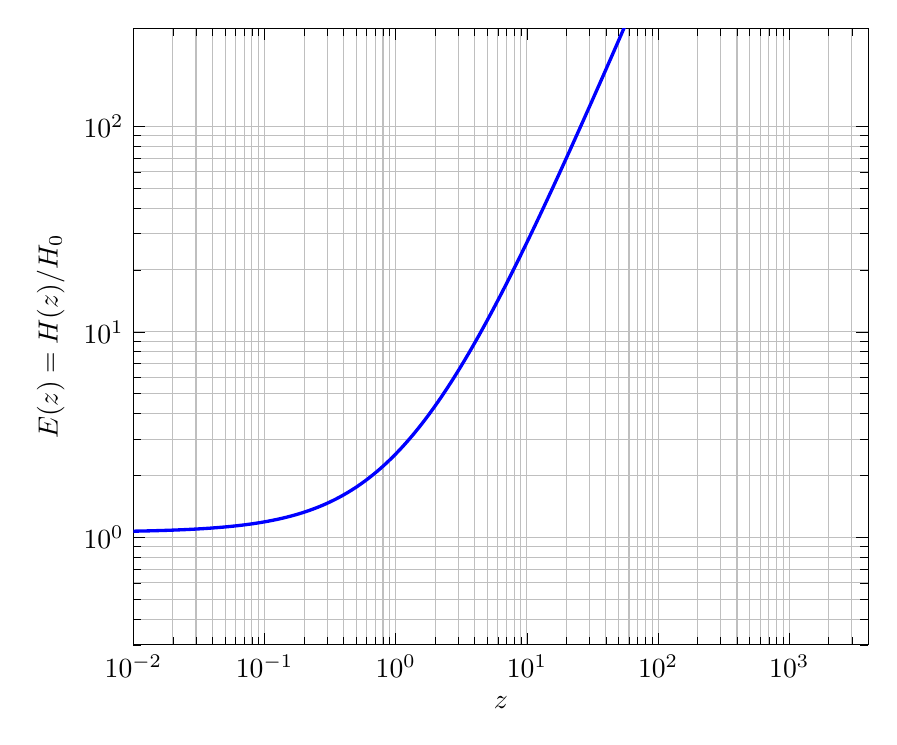
\begin{tikzpicture}
  \begin{axis}[
      width=0.9\textwidth,
      xlabel={$z$},
      ylabel={$E(z) = H(z)/H_0$},
      xmode=log, ymode=log,
      xmin=0.01, xmax=4000,
      ymin=0.3,  ymax=300,
      grid=both,
      tick style={black}]
    \addplot[very thick,blue,domain=0.01:4000,samples=240]
      {sqrt(4.2e-5*(1+x)^4 + 0.50*(1+x)^3 + 0.62*(1+x)^2)};
  \end{axis}
  \end{tikzpicture}
  %-------------------------------------------------------------
  \caption{Background expansion history $E(z)$ including radiation ($\Omega_{r0}=4.2\times10^{-5}h^{-2}$), matter ($\Omega_{m0}=0.50$), and the clock-field term ($\Omega_{\tau0}=0.62$).}
  \label{fig:BackgroundExpansion}
\end{figure}
